%
% fig-differenz.tex
%
% (c) 2025 Prof Dr Andreas Müller
%
\begin{figure}
\centering
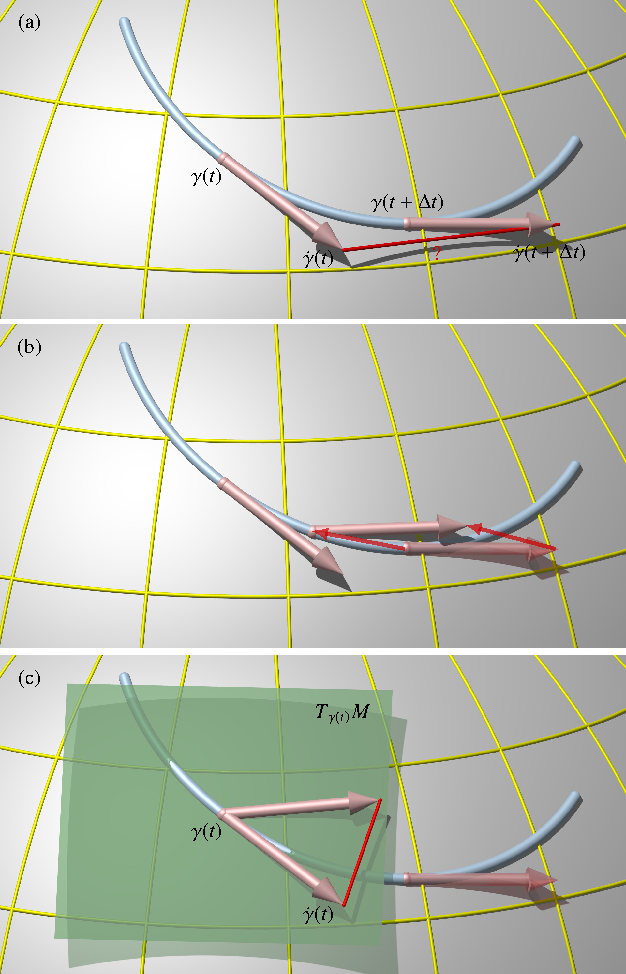
\includegraphics{chapters/100-zusammenhang/images/differenz.pdf}
\caption{Für die zweite Ableitung einer Kurve muss die Differenz
des Tangentialvektors $\dot{\gamma}(t)$ und $\dot{\gamma}(t+\Delta t)$
gebildet, werden.
Dies ist nicht möglich, weil die beiden Tangentialvektoren in 
verschiedenen Tangentialräumen liegen (a).
Der Tangentialvektor $\dot{\gamma}(t+\Delta t)$ muss daher zunächst
parallel in den Punkt $\gamma(t)$ transportiert werden (b).
Dann liegen die beiden Vektoren in der gleichen Tangentialebene
$T_{\gamma(t)}M$ und es kann die Differenz gebildet werden (c).
\label{buch:zusammenhang:fig:differenz}}
\end{figure}
